%%%%%%%%%%%%%%%%%%%%%%%%%%%%%% -*- Mode: Latex -*- %%%%%%%%%%%%%%%%%%%%%%%%%%%%
%% 09-07.tex --      IEEE Service Cup Paper
%% Author          : Philip Johnson
%% Created On      : Mon Sep 23 11:52:28 2002
%% Last Modified By: Philip Johnson
%% Last Modified On: Thu Jan 29 17:20:21 2009
%%%%%%%%%%%%%%%%%%%%%%%%%%%%%%%%%%%%%%%%%%%%%%%%%%%%%%%%%%%%%%%%%%%%%%%%%%%%%%%
%%   Copyright (C) 2009 Philip Johnson
%%%%%%%%%%%%%%%%%%%%%%%%%%%%%%%%%%%%%%%%%%%%%%%%%%%%%%%%%%%%%%%%%%%%%%%%%%%%%%%
%% 

%% Home page: http://iscc.servicescomputing.org/2009/
%% We are applying to the ``Service Computing Contest'' (for university professors/projects)

%% Should show how Hackystat explores ``new frontiers'' in SOA development.
%% 8 page limit for paper.
%% At most five students plus one professor.
%% Due date: February 20, 2009.  
%% Conference: July 7-10, 2009, Los Angeles.

%% Paper ID: 1122, http://confhub.com/MyPapers.php?cid=66

%% For ``peer review mode'', do:
%%   \documentclass[conference,compsoc,peerreview]{IEEEtran}
%% and
%%   \IEEEpeerreviewmaketitle  (after the abstract).

\documentclass[conference,compsoc,peerreview]{IEEEtran}
\usepackage[final]{graphicx}
\usepackage{cite}
\usepackage{url}
% uncomment the % away on next line to produce the final camera-ready version
% and uncomment the \thispagestyle{empty} following \maketitle
%\pagestyle{empty}

\begin{document}

\title{Experiences with Hackystat \\ as a service-oriented architecture}

\author{Philip M. Johnson \\
        Shaoxuan Zhang \\
        Pavel Senin \\
\em  Collaborative Software Development Laboratory \\
      Department of Information and Computer Sciences \\
      University of Hawai'i \\
      Honolulu, HI 96822 \\
      johnson@hawaii.edu \\
}


\maketitle
\IEEEpeerreviewmaketitle
%\thispagestyle{empty}

\begin{abstract}  % 200 words
Hackystat is an open source framework for automated collection and analysis
of software engineering process and product data.  Hackystat has been under
development since 2001, and has gone through eight major architectural
revisions during that time.  In 2007, we performed the latest architectural
revision, whose primary goal was to reimplement Hackystat as a
service-oriented architecture (SOA).  Hackystat Version 8 has now been in
public release for over a year, and this paper reports on our experiences:
the motivations that led us to reimplement the system as a SOA, the
benefits we have experienced from that conversion, and the new challenges
we now face as a result.
\end{abstract}


\section{Introduction}
\label{sec:intro}

Software engineering measurement is a compelling practice in principle. By
gathering data on the structure and quality of code, as well as the
behaviors of the developers as they build it, one can imagine obtaining
useful insight into the current state of development, better estimates of
what lies in store for the future, and ideas on how to improve current
practices and work artifacts.

The reality is that software engineering measurements are difficult to
obtain and difficult to interpret. To the extent that measurements are made
manually, this incurs overhead on the development staff which might seem
expendible when the schedule is tight.  Even when measurements are made,
useful insight and action is often difficult to obtain.  Is test case coverage of 70\%
good, bad, or someplace in between? Even if everyone agrees it is bad, what
exactly should be done, if anything?

Since 2001, we have been developing an open source framework for automated
collection and analysis of software engineering process and product data
called Hackystat (\url{http://www.hackystat.org/})
\cite{csdl2-06-06,csdl2-02-07}.  The goal of Hackystat is to provide an
extensible mechanism that can radically reduce the overhead associated with
collection of a wide variety of software engineering data, along with a
sophisticated toolkit of analyses that can facilitate useful
interpretation.  Over the years, Hackystat has been used in a wide variety
of application areas, including: classroom pedagogy \cite{csdl2-03-12},
inference of test-driven design practice \cite{csdl2-06-13}, software
engineering of high performance computing systems \cite{csdl2-06-08}, and a
telemetry-based approach to software measurement trend definition and
display \cite{csdl2-04-11}.

The Hackystat Framework is intended to be generic: it strives to be neutral
with respect to the platform, programming language and environment,
development process, and application domain.  We have not found this to be
a simple goal, and the architecture of Hackystat has undergone eight
significant revisions since 2001 in response to new application demands
upon the framework.

One of the most significant architectural revisions of all is the most
recent one, which occurred in 2007 when we migrated the Hackystat Framework
from a traditional client-server web application architecture to a
service-oriented architecture (SOA) using REST design principles.  This
required eight months of development and a rewrite of most of the system
(which by that time had grown to approximately 350,000 lines of code).

There are several reasons why we believe Hackystat is an interesting
example of a service oriented architecture.  First, it is a mature and
non-trivial system whose entire source code history is available and whose
conversion to SOA was motivated by concrete design issues.  Second, it
appears to be the first and only SOA-based software engineering data
collection and analysis system.  Other such systems (including SixthSense
Analytics, Programeter, Devcreek, SonarSource, ElectroCodeoGram, and EPM)
all have a client-server architecture.  Finally, Hackystat implements a
carefully designed combination of distributed computation, caching, and
pre-fetching that attempts to provide the flexibility and scalability of
SOA without sacrificing the performance of a simpler client-server
architecture.



The SOA version of Hackystat has been in public release for approximately
one year, and this has given us sufficient time to start to understand the
changes, both positive and negative, that have resulted from this move.
Section \ref{sec:motivation} discusses the shortcomings of our prior
Hackystat architecture which led us to reimplement the system in a
service-oriented manner.  Section \ref{sec:soa} introduces our current
service-oriented architecture and its features.  Section
\ref{sec:discussion} presents our experiences, both positive and negative,
with the SOA implementation.  Section \ref{sec:conclusion} summarizes our
conclusions and outlines some of our future architectural directions.


\section{Motivation for the Hackystat SOA architecture}
\label{sec:motivation}


\begin{figure*}[ht]
  \center
  \includegraphics[width=0.7\textwidth]{configurations5.eps}
  \caption{Two example Version 7 configurations}
  \label{fig:configurations}
\end{figure*} 

Hackystat architectural design decisions has always followed an ``agile''
approach of implementing ``the simplest thing that could possibly work''.
Since 2001, this has resulted in eight significant re-designs of the system
as it outgrew the constraints imposed by the previous architecture.  Some
might view this as a process-level bug, but we view it as a feature: we
could never have predicted in advance which application areas Hackystat
would be used in and the specific architectural pressures they would
create.  As a result, Hackystat's current implementation as a SOA
architecture is not based upon SOA being the current ``hot'' architecture,
but rather as a response to specific issues we were facing with the
previous version and the hope that SOA could address them.

To understand the costs and benefits of Hackystat Version 8, it is
important to know a little bit about its predecessor, Version 7.  First, by
the time of Version 7, Hackystat had grown to support software engineering data
collection and analysis in a variety of very different domains, including
Java-based classroom instruction, C-based high performance computing, Java
and Visual Studio-based test driven design inference, build system analysis
for NASA, a ``continuous'' approach to the Goal-Question-Metric paradigm,
and others.  To support sharing of overlapping functionality between these
domains, the 350 KLOC in the system were broken down into approximately 70
different modules.  While it was possible to build a release of Hackystat
containing all of these modules (and we did so for testing purposes), we
found that any particular domain of application was much better served by
supporting Hackystat ``configurations'', or builds of the system containing
a subset of all possible modules.

Figure \ref{fig:configurations} illustrates Hackystat modules, subsystems,
and configurations in Version 7.  It shows samples of modules (such as
``Standard'', ``HPC Experiment'', etc.) from two configurations: HPC and
Classroom.  Although only 10 modules are shown in the figure due to space
limitations, typical Hackystat 7 configurations contained from 30 to 60
modules.


Modules were assigned to one of four ``subsystems'' depending upon their
functionality: the ``Sensor'' subsystem contains modules providing software
``plugins'' to various tools; the ``SDT'' subsystem contains
implementations of structured sensor data called``sensor data types'', the
``Core'' subsystem provides basic client and server-side infrastructure,
and the ``App'' subsystem contains domain-specific analyses and user
interface facilities.


Each module in Hackystat was managed as a separate Subversion project, but
most could not be compiled individually. Instead, the build process would
take in a description of a Hackystat configuration as a list of modules,
and then compile those modules together into a functional client-server
application and run the set of tests associated with the included modules.
Each Hackystat module was required to indicate the other modules that it
depended upon so that the build process could sequentialize and resolve
dependencies.  If, during the build of a configuration, the system
encountered a module with a dependency that was not included in the
configuration list, an error was signalled.

Let's now turn to some of the problems we encountered with this approach to
modularity and flexibility within the confines of a client-server
architecture.

\subsection{System configuration binding time}

In the Version 7 architecture, we defined a system configuration as a list
of modules and then invoked the build system to produce a binary containing
those sets of modules.  This approach was the most straightforward way to 
build a single client-server system with a subset of all possible modules while 
still enabling testing and dependency resolution.

It did mean, however, that any user wanting to create a new configuration
adapted to their specialized needs would have to learn how to build the
system from sources. In Version 7, one could not take an existing binary
release and augment its functionality.  

\subsection{Complexity of build}

We discovered that our need for a configurable system building process
exceeded the standard capabilities of Ant, the canonical Java build system
tool.  To resolve this, we created a custom Hackystat build system
``wrapper'' around Ant.  This wrapper would take as input an XML
description of a Hackystat module and its dependencies, and generate a
number of Ant scripts that would correctly order the sequence of targets
for a particular configuration.

While the build system wrapper worked quite well, and actually automated
the generation of many thousands of lines of Ant build scripts, the problem
was that new Hackystat developers now needed to learn a custom and
unfamiliar build system approach in order to build Hackystat.  Furthermore,
not only developers of new Hackystat modules needed to learn this build
system, but even those who simply wanted to create a custom configuration
from existing modules needed to learn this system.


\subsection{Lack of access to ``intermediate'' analyses}

In the early stages of Hackystat development, sensor data was sent to a web
server, which performed relatively simple analyses over that data before
presenting that data to the user in a web page.  As the complexity of our
analyses increased, we found it useful to decompose some of them into
pipelines of smaller analyses.  For example, to obtain telemetry (trend)
data, the raw sensor data would first be analyzed into intermediate objects
called ``DailyProjectData'', which would then be input into the Telemetry
mechanism and further refined to produce the trends of interest.  As a
second example, the Test-Driven Design analysis would first organize the
raw sensor data into ``episodes'' which would then be input into a
rule-based system for classification with respect to TDD compliance.

Figure \ref{fig:subsystems} illustrates this aspect of the internal structure
of the server.  Raw sensor data ``percolates up'' through a series of analyses
to form increasingly higher level abstractions.  Some intermediate analyses 
(such as the SensorData analysis) could be used by multiple higher level analyses.

\begin{figure}[ht]
  \center
  \includegraphics{subsystems.eps}
  \caption{Version 7 subsystems and pipelines}
  \label{fig:subsystems}
\end{figure} 

One resulting problem with this pipeline is that though the intermediate
results were often interesting in their own right, they were not easily
accessed outside of the server-side processing mechanisms. Another problem 
resulted from caching, as discussed below in Section \ref{sec:caching}.

\subsection{Server-side and build language specificity}

The Hackystat framework is designed to be generic within the domain of
collection and analysis of software engineering process and product data.
It should run on all platforms, support sensors for arbitrary software
development tools and languages, and support analyses for a wide variety of
process and product measurement types.

The same language ``neutrality'' did not hold true when it came to the
framework itself.  Client-side sensors could (and were) written in a
variety of languages: Java, C\#, Emacs Lisp, etc. The server, however, was
a Java web application, and all analyses and user interfaces were required
to be written in Java and conform to the Hackystat web interface structure.

Similarly, the build system for Hackystat Version 7 was Ant, and the only
supported container for the server web application was Tomcat.

\subsection{UI rigidity}

To simplify UI development, Version 7 provided a high-level API for adding
new commands to the Hackystat web application interface which provided a
very standard look and feel.  Figure \ref{fig:commands} illustrates two
commands from Version 7 and their standardized look-and-feel.

\begin{figure*}[ht]
  \center
  \includegraphics[width=0.7\textwidth]{v7commands.eps}
  \caption{Two example Version 7 commands illustrating the common look and feel}
  \label{fig:commands}
\end{figure*} 

When first implemented, the user interface API saved time.  Though there
was a learning curve associated with it, the API enabled the set of modules
in a given configuration could contribute its own set of commands to the
user interface.  It also guaranteed that all commands would exhibit the
same user interface. Finally, we implemented an API that made it simple to
programmatically invoke commands in the user interface from test code.

By the time of Version 8, we began to feel that the user interface standard
was also a straightjacket: Hackystat's architecture was effectively
``frozen'' with a single user interface style and both the build system and
test system (as well as actual UI code) would need to be changed
significantly in order to support experimentation with alternative user
interfaces.

\subsection{Cache thrash}
\label{sec:caching}

In the Telemetry application, it was not uncommon to regularly request an
analysis that might display 30 or 40 trend lines for a set of software
projects over the last several months. Such a request could easily involve
the processing of hundreds of thousands of raw sensor data
instances. However, many of those trend lines might require access to the
raw same sensor data, and many if not most of the trend line components
might involve computations that were performed previously the last time the
analysis was requested.

We quickly discovered that a naive implementation of telemetry could
easily take several hours to perform common types of analysis, but that our 
``pipeline'' form of analyses lent itself naturally to caching.

The basic idea is simple: use caches to store the results of intermediate
computations.  Referring again to Figure \ref{fig:subsystems}, we
implemented a cache for Sensor Data (which avoided to cost of going to the
database), a cache for Daily Project Data instances (which avoided the cost
of re-processing Sensor Data), and a cache for Episodes (which again
avoided the cost of re-processing Sensor Data).

The introduction of multiple caches worked extremely well for a while.
Computations which could have taken hours now took only seconds or minutes.
Unfortunately as the system continued to grow in size and complexity,
caching began to create problems of its own.  The millions of sensor data
instances in a Hackystat sensor data repository meant that we could not
simply cache everything; we needed to limit the size of the various caches.
As the number of caches for different types of intermediate objects
increased, we started to see evidence of ``cache thrash'': one cache
appeared to be discarding objects just as another cache would be requesting
them. Tuning the various caches to maintain the right size and work
effectively with each other was a very difficult performance analysis.

\section{Hackystat as SOA}
\label{sec:soa}

To summarize, Hackystat's original client-server architecture worked well
when Hackystat processed relatively few kinds of data in relatively few
kinds of ways for a relatively small number of users.  We hypothesize that
the prior architecture would have scaled well, at least for a while, if
growth had been restricted to just one of these three dimensions.

Unfortunately, the system grew in scale along all three of these dimensions
simultaneously.  We attempted to manage its size and complexity while
staying within the basic client-server architectural model in several ways:
by a custom module system to support configurations; by pipelining analysis
processing; by caching; and by high level APIs for the user interface,
build system, and testing.

By 2007, however, we realized that we had designed ourselves into a
corner: the system structure was well suited to a certain performance
load and set of application domains, but the features that achieved that
also actively prevented us from other kinds of extensions and enhancements.

After a month of discussion, we halted all development on the Version 7
code base and started over with a new architectural paradigm: a RESTful
service-oriented architecture.  Figure \ref{fig:soa} illustrates the
ten services now available or in active development in Version 8.

\begin{figure*}[ht]
  \center
  \includegraphics[width=0.7\textwidth]{soa.eps}
  \caption{Services now available or in development for Hackystat Version 8}
  \label{fig:soa}
\end{figure*} 

A comparison of Figure \ref{fig:soa} with Figure \ref{fig:subsystems}
reveals the major similarities and differences between the old
client-server architecture and the new service-oriented architecture.
First, Hackystat Version 8 retains a similar kind of pipelined, incremental
approach to analysis that was present in Version 7. This is illustrated by
the presence of uniformly upward pointing arrows in both Figures.  In both
versions, raw sensor data is stored in a database and ``percolates upward''
through various kinds of analyses toward a user interface.

However, in Version 8 there is no longer a ``box'' around the analyses,
indicating that instead of a single server, Hackystat now consists of a
number of cooperating services, some of which correspond relatively
directly to analysis subsystems within the old system (such as SensorBase,
DailyProjectData, and Telemetry), and others of which are brand new:
ProjectBrwoser, Tickertape, and TrajectoryViewer.

In Figure \ref{fig:subsystems}, the arrows essentially correspond to Java
method invocations within a single process that illustrate data and control
flow in the system.  In Figure \ref{fig:soa}, the arrows still illustrate
data and control flow, but rather than Java method invocations, the arrows
correspond to HTTP calls designed according to REST (Representational State
Transfer) principles \cite{Fielding02}. 



\section{Pros and cons of SOA}
\label{sec:discussion}

Here we discuss how the SOA architecture addressed all of the issues we encountered in Section \ref{sec:motivation}, and what new issues we are confronting. 

Pro: Restart a single service without bringing down entire system.

Con: Loss of compile-time structural consistency checking for sensor data types.

Note: non-real time nature; don't need data to be synchronized down to the second. 

No appreciable change in lines of code. 

Natural distribution of services across machines. 

Replication of services possible.

\section{Conclusions}
\label{sec:conclusion}

Conclusions and future directions. 


\bibliographystyle{IEEEtran}
\bibliography{tdd,zorro,csdl-trs,hackystat,psp}
\end{document}











